%%%%%%%%%%%%%%%%%%%%%%%%%%%%%%%%%%%%%%%%%%%%%%%%%%%%%%%%%%%%%%%%%%%%%%%%%%%%%%%%
% TODO:
% Make is flow smoother and strike the main components necessary to build a 
% strong middleware system

%%%%%%%%%%%%%%%%%%%%%%%%%%%%%%%%%%%%%%%%%%%%%%%%%%%%%%%%%%%%%%%%%%%%%%%%%%%%%%%%
% begin introduction

\chapter{Introduction} %{{{
  \section{Motivation} %{{{
    This dissertation presents a novel distributed optimization algorithm designed
      to find and optimize solutions for highly nonlinear and complex systems.
    The algorithm presented is the Persistent Distributed Agent-Based Genetic 
      Algorithm (PDABGA) and this dissertation applies the algorithm towards 
      generating and optimizing a robotic gait for a multi-jointed compound
      modular robot.        
    Generating and optimizing gaits for large robotic systems will become more
      and more important as robotic systems become large and complex. 
    As demonstrated by the Mars rovers, robotic systems have also been proven
      to be viable solutions toward space exploration.
    As the range of exploration extends farther out into the Solar System, 
      communications and direct remote control of robotic systems will likely
      become infeasible.
    In order to fulfil exploration missions, robots will need more autonomy and
      will have to adapt to their environment, be it through self-reconfiguration,
      gait generation, multi-robot cooperation, or other creative methods.

    The PDABGA presented here is intended to be a tool to help a team of robots
      figure out how to complete a complex task by pooling their computational
      resources. 
    The PDABGA is distributed, decentralized, persistent, and extremely fault
      tolerant so that it may run effectively on systems such as networked teams
      of robots. 
    These attributes allow the PDABGA to tackle very large optimization problems
      over long periods of time while efficiently utilizing all available CPU
      resources.
    Specifically, tasks such as gait generation and optimization for mobile
      modular robots of arbitrary morphology is a problem currently impossible
      to solve using analytical methods due to the non-linear and nonholonomic
      nature of non-rolling robotic gaits. 
    Therefore, such a problem presents a perfect scenario for usage of the PDABGA.

    %It is especially useful if the solution space is large and it is difficult
    %  or impossible to analyze the task with analytical methods, but a
    %  simulation of the task can be implemented.
  %}}}

  \section{A Review of Genetic Algorithms} %{{{
    Genetic algorithms were first conceptualized in the 1960’s by John Holland as a
      method of optimizing complex problems \cite{Goldberg1988}. 
    Genetic algorithms search for an optimal solution to a problem by
      investigating a pool of candidate solutions and spawning more candidate
      solutions through biologically inspired processes of selection,
      chromosome crossover, and mutation. 
    Many variants of the original genetic algorithm have now been investigated
      such as genetic programming \cite{Koza1994, Banzhaf2000}, a method of using
      similar natural selection techniques to generate computer code rather than
      a chromosome. 
    Various chromosome selection and crossover algorithms, and structured
      genetic algorithms have also been studied. 
    %Research into the simultaneous usage of multiple processors and/or multiple
    %  networked computers has also been performed to increase the speed of
    %  convergence.

  \subsection{Structured Genetic Algorithms} %{{{
    Structured GAs are similar to the canonical GA with additional rules regarding
      mate selection, population management, or other aspects of the canonical GA. 
    It has been argued that the standard GA is prone premature convergence, in
    which a population settles on a local minima \cite{Fogel1994}. 
    Structured GAs attempt to mitigate these issues by enforcing rules about
      how the population interacts with each other, typically based on real world
      phenomena. 
    Examples of structured GAs include the island model, cellular GAs, and
      various GAs which depend on certain attributes of the individuals of a
      population.

    In the island model GA, separate populations evolve independently. 
    At certain generational intervals, individuals may migrate from one island
      to another, spreading genetic material \cite{Whitley1999, Artyushenko2009}.
    Since each island evolves separately for the majority of its lifetime, it
      is less likely for them to settle on the same local minimum, and thus more
      likely for at least one population to converge on the global minimum. 
    Also, because of the limited communication between islands, this structure
      is ideally suited to run in a distributed execution environment, such as a
      cluster of networked computers.

    In the cellular model GA, each individual is indexed on a 2-d or 3-d toroidal
      grid. 
    In general, each individual is only allowed to interact with direct
    neighbors or nearby individuals \cite{Alba2005}. 
    In this model of structured genetic algorithm, various areas of the
      population space may converge on separate minima since the spread of
      genetic material across the population is limited to a certain distance per
      generation.

    Various other methods of structuring populations of GAs exist, including
      multinational evolutionary algorithms \cite{Ursem2000}, religion based
      evolutionary algorithms \cite{Thomsen2000}, social interaction models
      \cite{Al-madi2008}, tracking individual ages and life spans
      \cite{Kubota1997}, and many more.

    %Initially, genetic algorithms were run on a single computer with a single
    %  population of potential solutions. 
    The trend now has been to distribute and parallelize the process
      \cite{Tomassini1999, DAmbrosio2006, Kim2006, Cantu-Paz2007, Cantor2010}. 
    Distributed and structured genetic algorithms are able to utilize the
      computational power of multiple geographically separate computers
      simultaneously to solve a single problem. 
    Many distributed genetic algorithm structures are also better able to avoid
      local minima and premature convergence \cite{Artyushenko2009, Alba2005}.
    However, since many distributed genetic algorithms are only intended to run
      for no more than a few hours or days at a time, all typically use a central
      controller, which presents a single point of failure. 
    %}}}

  \subsection{Distributed/Parallel Genetic Algorithms} %{{{
    Distributed and parallel genetic algorithms are two related but distinct
      paradigms. 
    Usage of the term ``parallel'' in the context of GAs has come to imply a
      multi-threaded or multi-process application which utilizes many CPUs on a
      single computer, where each thread might share a single memory space, or
      separate processes use inter-process communication to interact. 
    On the other hand, the term ``distributed'' has come to imply a GA which
      runs on many separate individual computers which connect together through a
      network, such as the Internet. 

    While these two paradigms are similar in that processes run simultaneously,
      there are several major differences.
    First, on a parallel system, each CPU can be considered to be highly
      fault-tolerant.
    It is unlikely for a single CPU to fail without the entire computer failing.
    Furthermore, the CPUs are typically highly homogeneous.
    In the distributed case, if the computers are geographically remote, they
      can encounter individual network shortages, power outages, etc.
    Also, because multi-threaded applications on a parallel machine can share a
      memory space, the available communication bandwidth between threads is
      typically orders of magnitude higher than that available to processes
      communicating over the Internet. 
    As such, the design and implementation of distributed GAs must take into
      account the fault tolerance of the algorithm to failing nodes and low
      bandwidth while parallel GAs may not need to worry about those issues.

    In the following descriptions of structured GAs, only the distributed versions
      will be considered. 
    With the advent of the Internet and Cloud Computing, large supercomputers
      have begun to fall out of favor among the high-powered GA community.
    Hyper parallel super computers are extremely expensive and are typically only
      owned by large entities, such as universities. 
    Even at universities, it can be difficult to reserve time on these
      supercomputers. 
    Current trends indicate that highly scalable massively distributed
      evolutionary algorithms will gain wider and wider usage.

    The suitability of each of the structured genetic algorithms for parallel
      and distributed computing varies. 
    In the simplest case, the canonical GA may be implemented in a distributed
      manner simply by running the objective function in parallel
      \cite{Schutte2004}. 
    In the distributed version of the canonical GA, a single master entity
      controls the operation of all of the individuals of the population
      \cite{Luque2005}. 
    This indicates that there must be frequent communication between the
      individuals and the algorithm which handles selection and reproduction. 
    As such, this type of algorithm is best suited to either a single computer
      with many processors in a parallel GA so that the algorithm can share a
      memory space, or a cluster of homogeneous computing nodes on a very fast
      network in a distributed GA. 

    The island model is ideally suited to run in a distributed environment where
      each processing node handles a single island of the GA. 
    Each island runs its own GA in the standard sequential manner. 
    The island model is considered a course-grained model \cite{Cantu-Paz1998}
      due to the limited communication between the islands which happens only
      during migration events. 
    Because of the limited communication among islands, there is minimal
      overhead due to network communications. 
    However, because of the synchronized nature of processing generations in
      the island model, it is better suited to homogeneous computing
      environments. 
    In a highly heterogeneous computing environment, the algorithm must wait
      for the slowest node to finish its computations before entering the
      migration phase \cite{Desell2010}.

    The cellular GA structure can be considered a stereotypical fine-grained
      model of a distributed GA \cite{Cantu-Paz1998, Schoneveld1996}. 
    In this case, each distributed computing node is typically placed on a
      virtual 2-D or 3-D toroidal grid and handles only a small population or
      single individual. 
    During the reproduction phase, each computing node is only allowed to
      communicate with its grid neighbors. 
    These algorithms are suited to optimization problems where calculation of
      the fitness function is long compared to the time of network communication,
      and the required population to generate good results is
      relatively low. 
    In cases where the objective function is fast, the computing time will be
      dominated by network communications, and high populations require a high
      number of computational nodes, which may be expensive or impossible to
      attain. 
    Also, these algorithms are typically run in a synchronous manner, which
      makes them prone to the same drawbacks as the synchronous island GA
      structure. 

    Additionally, there are a number of vast, super-scalable asynchronous
      approaches which are suitable for widely distributed highly heterogeneous
      computing environments. 
    Asynchronous approaches have been shown to be more fault tolerant than 
      synchronous methods while maintaining the performance of synchronous approaches
      \cite{Lewis2009}. 
    The MilkyWay@Home project is a large persistent distributed evolutionary
      algorithm which utilizes volunteered computing power from thousands of
      networked peers to find the substructure of the Milky Way galaxy
      \cite{Cole2010}. 
    The MilkyWay@Home project builds on other Volunteer computing projects
      created the last decade such as SETI@Home \cite{Anderson2002}, ``The Great
      Internet Mersenne Prime Search'' \cite{mersenne_website} and
      ``Distributed.net'' \cite{distributednet_website}. 
    These projects all use grid computing middleware such as the Berkeley Open
      Infrastructure for Network Computing (BOINC) \cite{Anderson2004} to
      organize the large volunteer computing networks. 

    Recently, there has also been research towards agent based and peer-to-peer
      evolutionary algorithms. 
    These types of algorithms are intended to have similar persistence and
      scale as the grid computing frameworks, but without a central controller.
    Furthermore, because the agents are autonomous, they may be able to
      utilize distributed CPU power more effectively \cite{Laredo2010, Lee2011}. 
    The work presented in \cite{Lee2011} is analogous to an asynchronous
      island-type distributed GA where each agent controls a subpopulation of
      candidate solutions. 
    The agents are able to migrate to remote hosts depending on a number of
      factors, such as the availability of CPU time or memory. 
    However, the algorithm uses a central controller which manages the overall
      function of the algorithm.

    The EvAg framework presented in \cite{Laredo2010} demonstrates the feasibility
      of a massively decentralized persistent agent-based genetic algorithm. 
    The EvAg framework is analogous to an asynchronous cellular GA. 
    Each agent represents a single candidate solution in the EvAg framework and
      maintains its own list of neighbors for reproduction.  
    The agents used in the EvAg framework are not mobile, however, and is
      intended to run on widely distributed PC networks. 
    The EvAg system has been shown to generate good results while using an ad-hoc
      decentralized population distribution.
  %}}} subsection
  %}}} section

  \section{A Review of Mobile-Agent Systems} %{{{
    % FIGURE --------------------------------------------------
    \begin{figure}[!ht]
    \begin{center}
       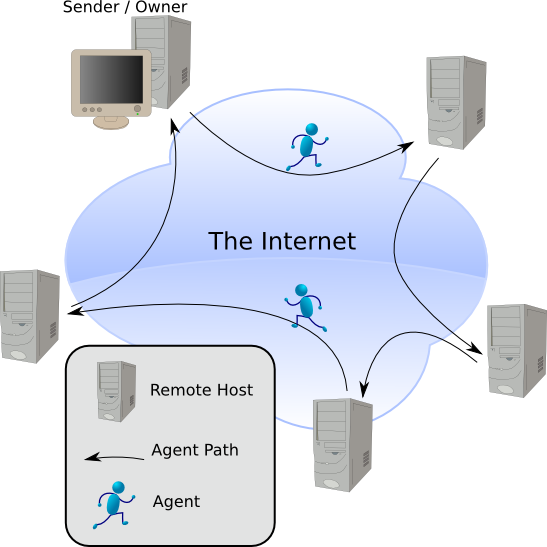
\includegraphics[width=3in]{figures/internet_agencies}
    \end{center}
    \caption{\label{fig:internet_agencies}A mobile agent visiting hosts
    on the Internet.}
    \end{figure}
    % END FIG -------------------------------------------------

    Mobile Agents are essentially autonomous computer programs which may
    migrate mid-execution to other hosts. 
    Figur \ref{fig:internet_agencies} shows a mobile agent visiting a number
      of geographically separated hosts in a sequential manner. 
    Various mobile agent platforms have been developed over the years in
    various languages and computing environments. 
    They have been successfully used in a variety of engineering applications
    such as manufacturing \cite{DiStefano2008, Nestinger2010}, computer vision
    \cite{Nestinger2010b}, distributed sensor networks \cite{Fok2005, Wu2001},
      and structural health monitoring \cite{Taylor2009}. Some popular agent
      systems include Mole \cite{Baumann2002}, Java Aglets \cite{Lange1998},
      Ara \cite{Peine2002}, Tacoma \cite{Johnansen2002}, Concordia
      \cite{Wong1997}, D’Agents \cite{Gray2002}, JADE \cite{Bellifemine2008},
      PEERWARE \cite{Cugola2001}, MARS \cite{Cabri2000}, and
      Mobile-C \cite{Chen2006, Chou2010, mobilec}. 
    Among these mobile agent platforms, JADE perhaps enjoys the most general
      usage. 
    However, JADE is implemented in JAVA and is not directly capable of
      accessing low level function calls when running on embedded systems. 
    Of these agent platforms, Mobile-C is the only platform capable of running
    C/C++ agents which are directly capable of calling low level system calls
      for purposes of robotic control \cite{Nestinger2010}, and has been
      successfully tested on the iMobot \cite{Ryland2010, Ko2010}, a modular
      robot.

  %}}} section

  \section{A Review of Modular Robots}

    Modular robotics is a class of robotics where robots are composed of smaller
      robotic units, each with their own actuation and sensors. 
    Many designs for modular robotic systems have been presented over the years. 
    Atron \cite{Jorgensen2004, Christensen2006} is a simple self-reconfigurable
      modular robotic system in which each module has only a single degree of
      freedom.
    Similar to Atron, Molecubes \cite{Zykov2007} is another example of a
    self-reconfigurable 1 degree-of-freedom robot. 
    Molecubes, however, can support more than one type of module, and other
      modules, such as gripper modules, also exist. 
    The MTRAN \cite{Murata2002}, Superbot \cite{Shen2006, Salemi2006}, and iMobot
      \cite{Ryland2010} share similar morphologies, except they have two, three, and
      four degrees of freedom per module, respectively. 
    Of the three, only the MTRAN and Superbot modules are capable of
      self-reconfiguration, but the iMobot modules are more mobile as single
      modules. 

    Recently, modular robots have become available to the general public. 
    The Molecubes project is an open source project which enables capable researchers
      to build their own set. 
    However, Molecubes are not available pre-assembled to the general public,
      and the assembly process is not straight-forward. 
    Cubelets \cite{cubelets_website} are a commercially available modular robotic system
      geared towards education among young children. 
    However, due to the simplicity of the Cubelets robotic system, the robots
      tend to be highly static and dynamically uninteresting. 
    Finally, a modular system known as Mobots have recently entered the market
    \cite{barobo_website}. Mobots are based on the
      iMobot\cite{Ryland2010} and share similar design features. 
    Compared to cubelets, each module has a high range of motion which makes it
      a very complex, dynamic system. 
    Mobots are easily configurable to many different configurations as shown in
      Figure \ref{fig:mobot_modules}, and are commercially available
      fully-built and ready to use.

    % FIGURE --------------------------------------------------
    \begin{figure}[!ht]
    \begin{center}
    \subfigure[A single Mobot module.] {
       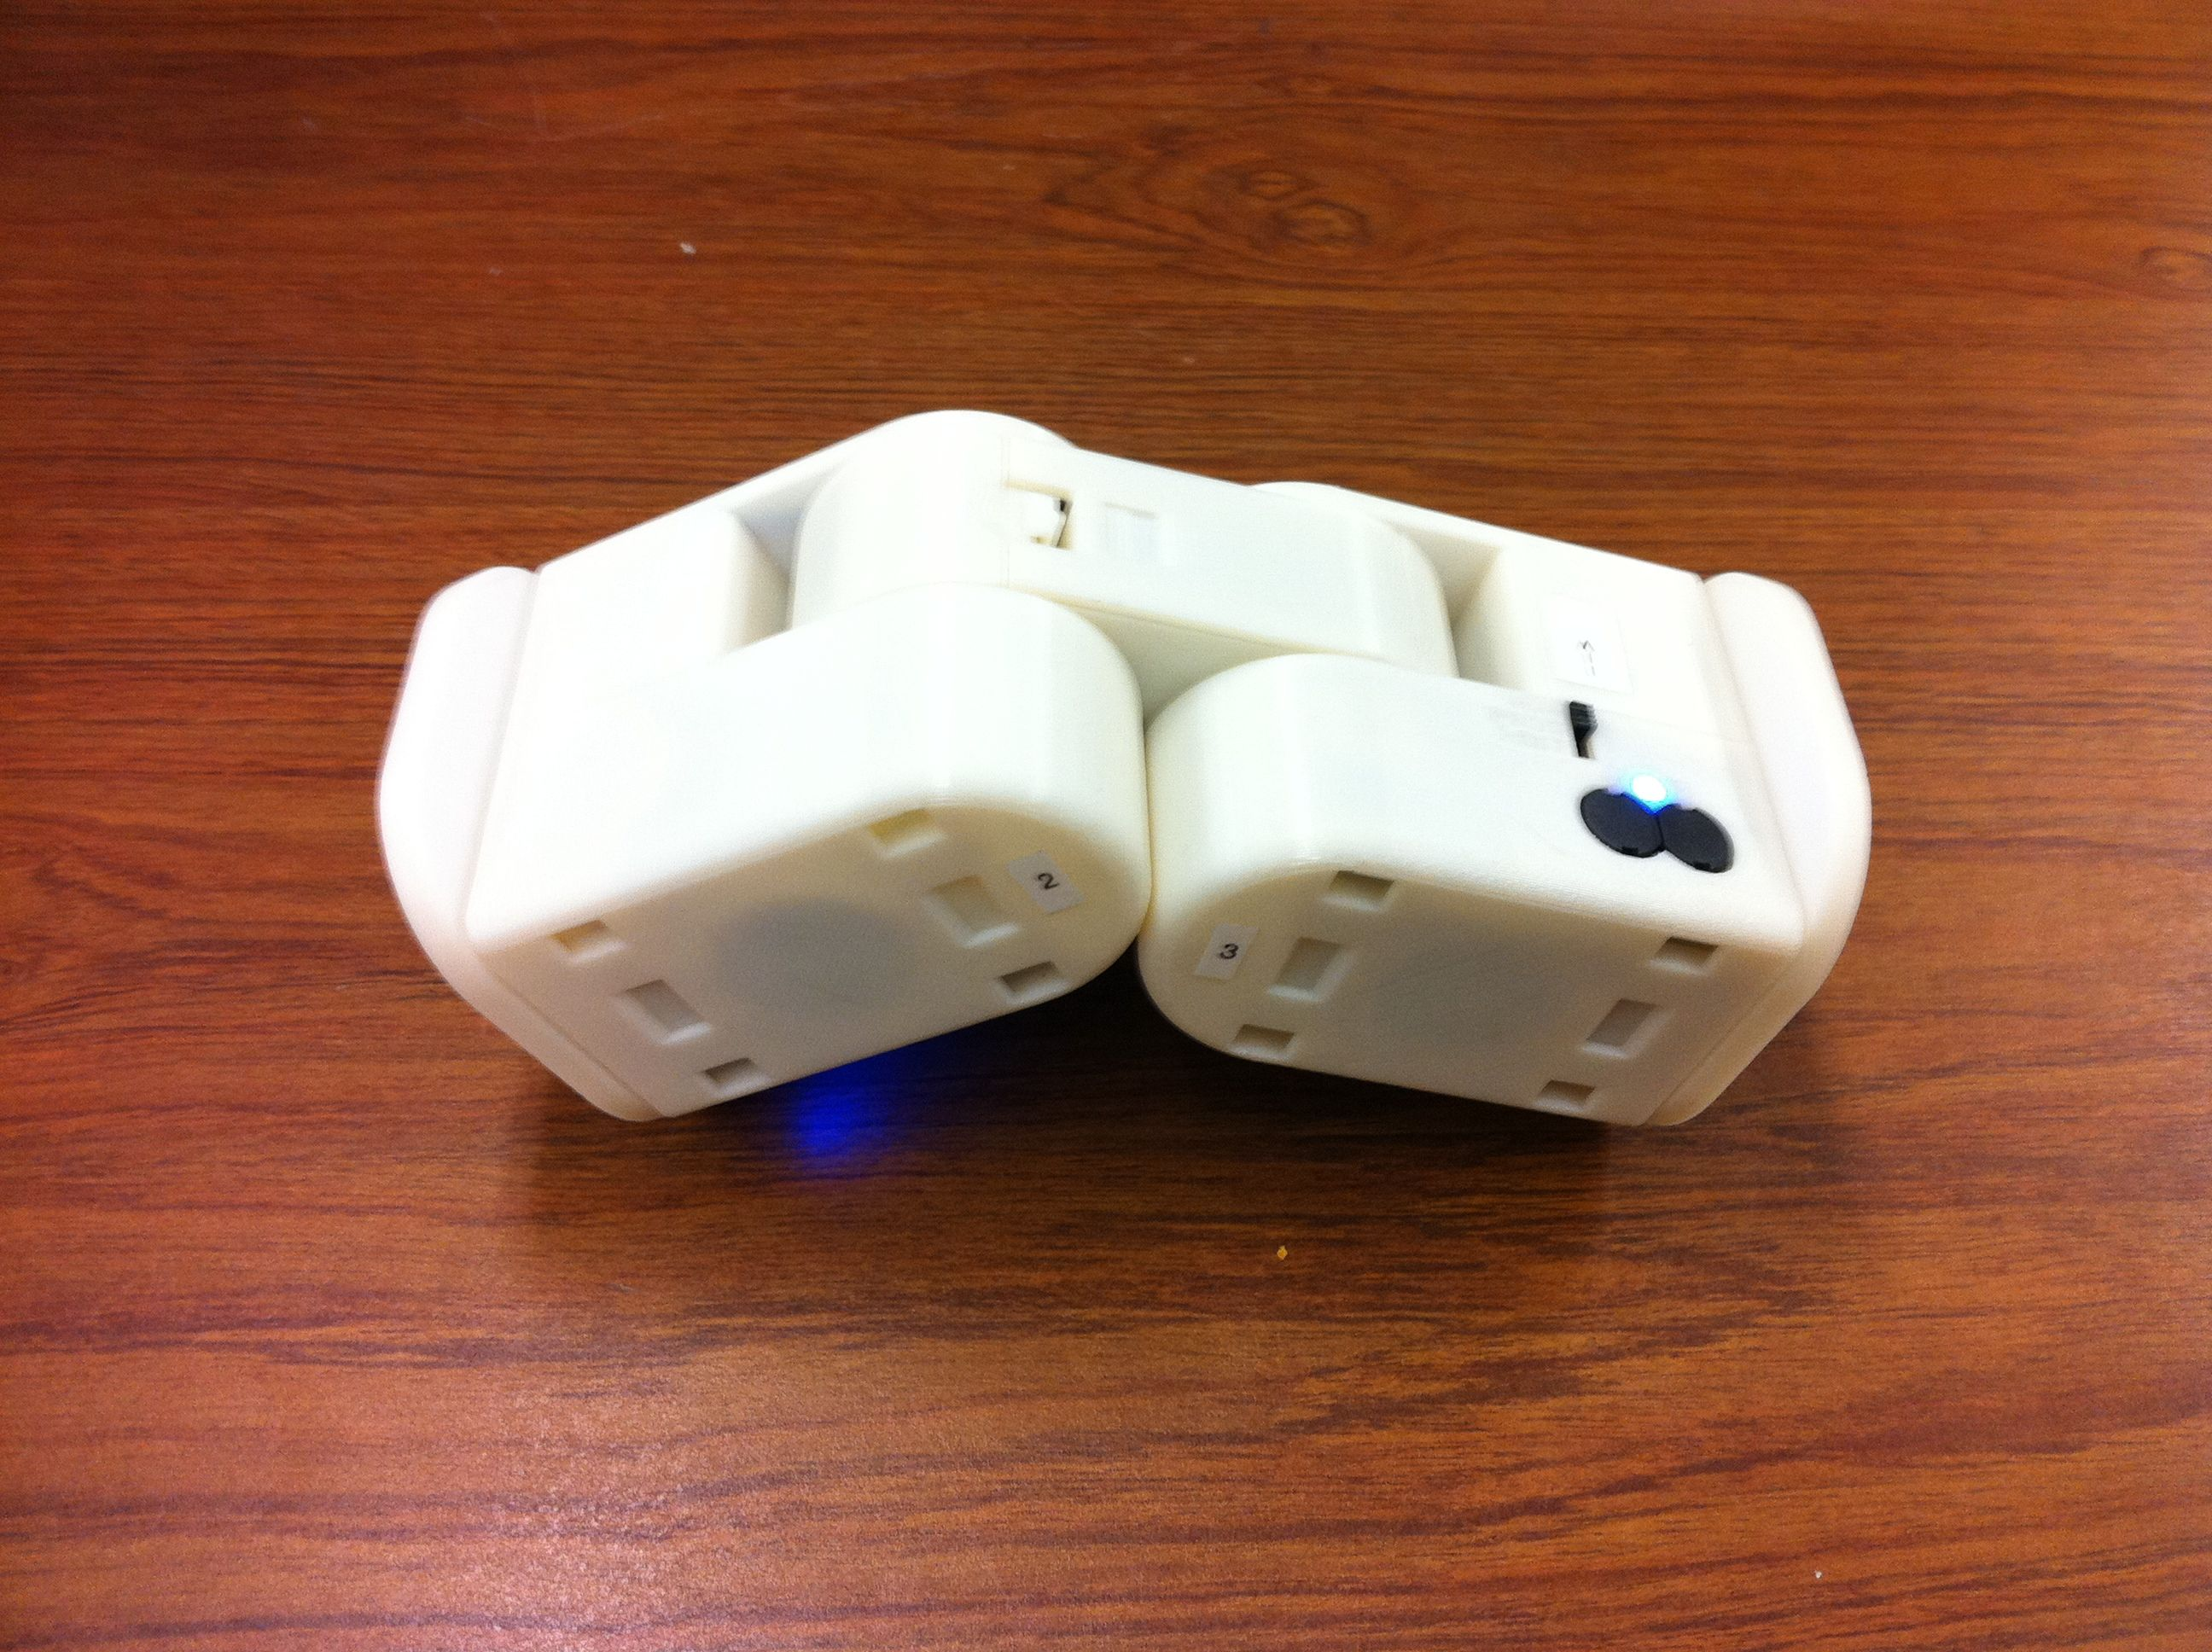
\includegraphics[width=2in]{figures/inchworm2}
    }
    \subfigure[Two attached Mobot modules.] {
       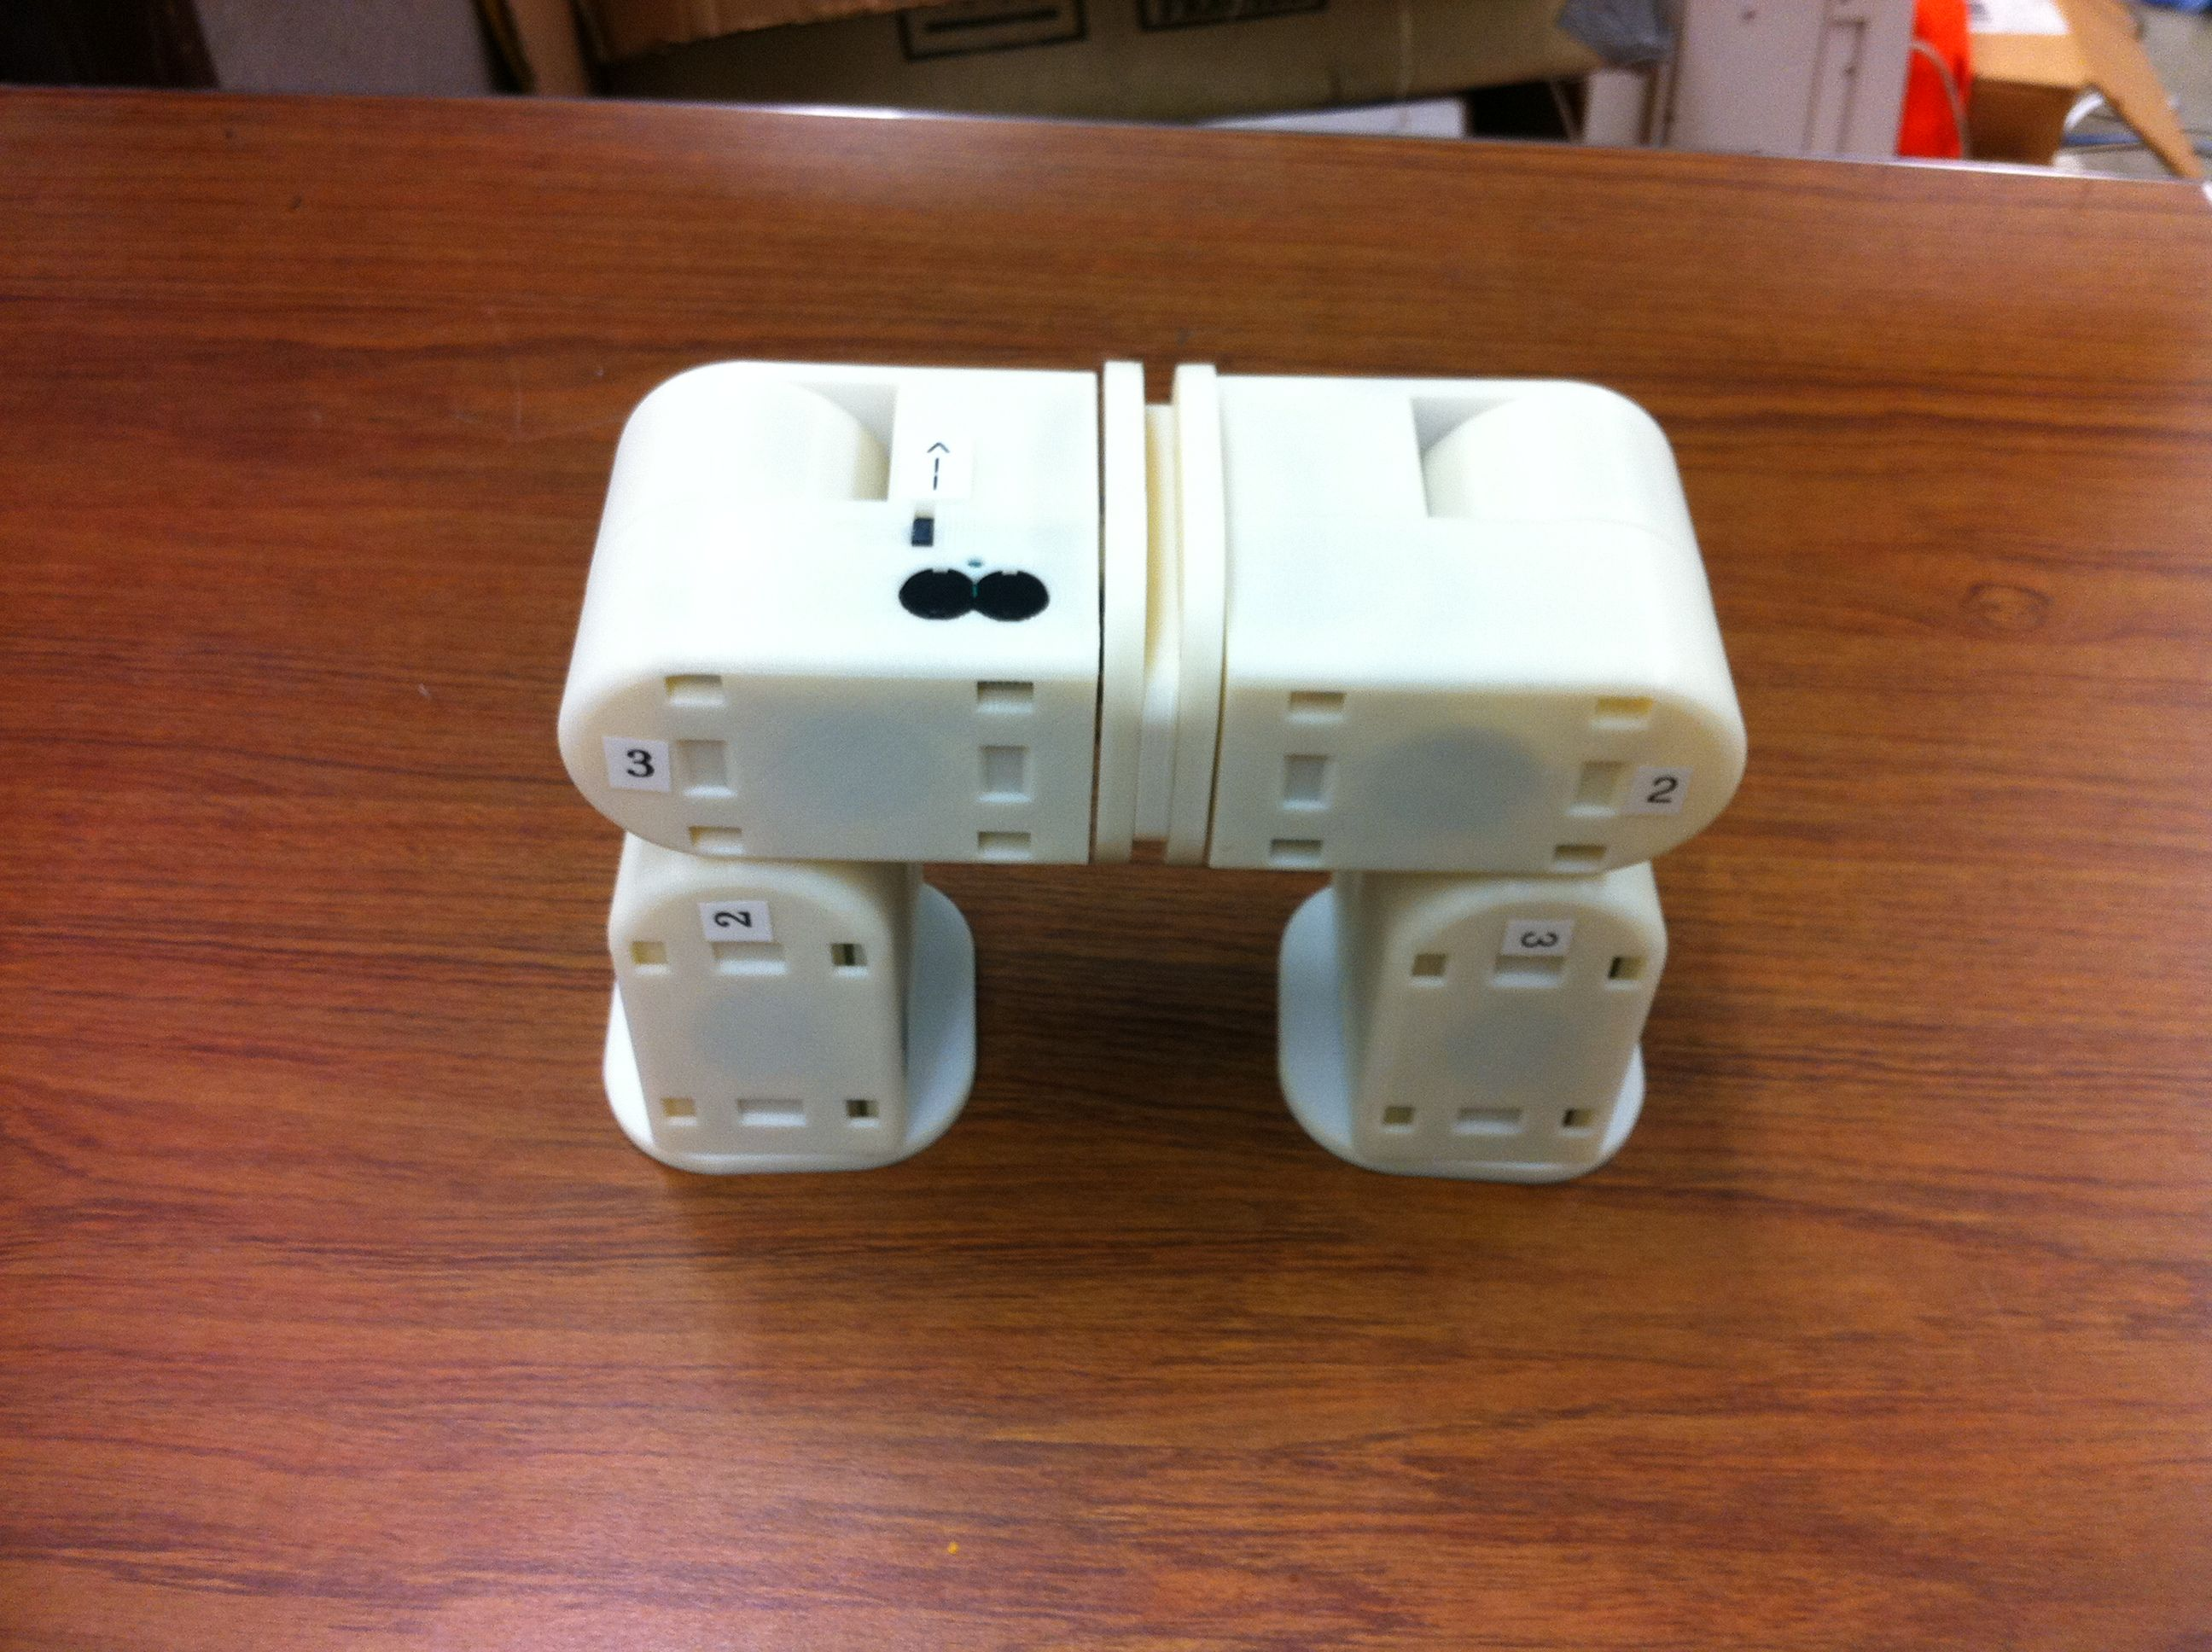
\includegraphics[width=2in]{figures/lift2}
    }
    \end{center}
    \caption{\label{fig:mobot_modules}Mobot modules.}
    \end{figure}
    % END FIG -------------------------------------------------

  \section{Robotic Gait Generation and Optimization}
    A common research topic among many modular robotic systems is the
      generation of robotic gaits. 
    Traditionally, robotic gaits were designed by humans and implemented as
      gait tables \cite{Yim2000, Kamimura2001}. 
    Hands-on methods of generating gait tables have also been investigates,
      such as ``pose teaching'' \cite{Ryland2010}. 
    Pose teaching for modular robots is analogous to ``lead-by-the-nose''
      teaching for robotic arms where the user physically manipulates the robot
      through a series of desired poses or motions.  
    However, gait tables require central control, and are not especially fault
      tolerant. 
    Furthermore, as modular robotic systems get large, the increasing degrees
      of freedom of the robot make pose-teaching unmanageable. 
    Research was eventually steered towards distributed control laws, such as
      phase automata \cite{Zhang2003}, and neural networks and similar control
      methodologies \cite{Canavier1997, Inagaki2006, Derosa2008}. 
    Using these strategies, unique gait patterns have been developed which do
      not require a central controller \cite{Sastra2009}.

    Much research has also been directed towards the automated generation of
      gaits rather than relying on human design. 
    In cases where an automated robotic system is incommunicado, it is
    infeasible to rely on human interaction when controlling robots. 
    When modular robotic systems get large, designing a gait for dozens or even
      hundreds of modules becomes a daunting task.
    Furthermore, there is no indication that the human-designed gaits are
      optimal in any way. 
    For robotic systems where the geometry of the robot is well known, there
      exist analytical methods for gait generation \cite{Weingarten2004}.
    However, as soon as robot morphologies become arbitrary and complex,
      analytical methods become hard. 
    Calculating the inverse kinematics for a complex compound mobile robot can
      be hard or impossible. 
    Thus, rather than pursuing analytical methods, current research on gait
      generation for complex robots has levied the power of computer simulations
      and evolutionary algorithms to generate gaits. 
    It has been shown that even gross simplifications of a robot in a simulated
      environment may still be useful towards generating useful controllers and
      gaits \cite{Jakobi1995, Jakobi1998, Bongard2004, Lipson2006,
      Zagal2007}. 
    It has been shown that using a combination of simulated environments and
      testing on physical robots can produce effective real-world gaits
      \cite{Zagal2007, Koos2010}. 


  \section{Approach} %{{{
    The basic strategy behind the design of the PDABGA is to imbue mobile 
      agents with the core principles of evolutionary algorithms; survival 
      of the fittest, genetic crossover, and mutation. 
    Agents and agency networks themselves tend to be highly distributed, 
      decentralized, and very fault tolerant. 
    The agents are executed on multiple agencies distributed across a 
      decentralized network and perform their own fitness calculations, mate
      selection, crossover, and breeding. 
    Helper agents running on each agent manage population sizes and other
      tasks.   
    The agents and agencies are implemented using Mobile-C, an agency
      supporting C/C++ agents which has been revamped and heavily upgraded during
      the course of this research.

    While the PDABGA is applicable in a wide range of areas,
      this dissertation will use the algorithm towards generating and
      optimizing a robotic gait for a modular robotic system.
    As robots computation becomes cheaper and cheaper, modular robots
      consisting of hundreds or even thousands of modules will become 
      more and more commonplace.
    These modular robotic systems represent a highly suitable use case scenario
      for the PDABGA. 
    Modular robotic systems are dynamically complicated which can exclude the
      possibility of designing and optimizing gaits analytically. 
    They have many distributed computational resources with each module acting
      as a computational load.
    However, Modular robotic systems also tend to be highly faulty, where
      individual nodes may fail catastrophically and without warning.

    %}}} section


% end introduction }}}
%%%%%%%%%%%%%%%%%%%%%%%%%%%%%%%%%%%%%%%%%%%%%%%%%%%%%%%%%%%%%%%%%%%%%%%
